% This file was created by tikzplotlib v0.8.7.
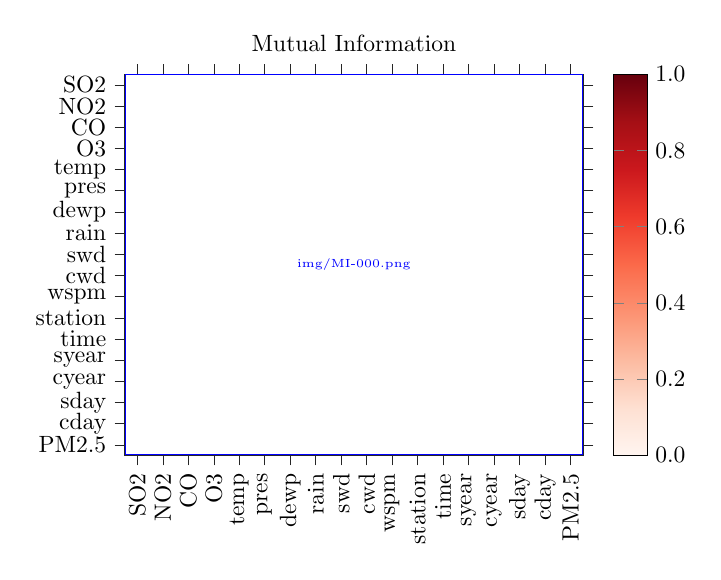
\begin{tikzpicture}[scale=0.85]

\begin{axis}[
axis line style={white!15.0!black},
colorbar,
colorbar style={ytick={0,0.2,0.4,0.6,0.8,1},yticklabels={0.0,0.2,0.4,0.6,0.8,1.0},ylabel={}},
colormap={mymap}{[1pt]
  rgb(0pt)=(1,0.96078431372549,0.941176470588235);
  rgb(1pt)=(0.996078431372549,0.87843137254902,0.823529411764706);
  rgb(2pt)=(0.988235294117647,0.733333333333333,0.631372549019608);
  rgb(3pt)=(0.988235294117647,0.572549019607843,0.447058823529412);
  rgb(4pt)=(0.984313725490196,0.415686274509804,0.290196078431373);
  rgb(5pt)=(0.937254901960784,0.231372549019608,0.172549019607843);
  rgb(6pt)=(0.796078431372549,0.0941176470588235,0.113725490196078);
  rgb(7pt)=(0.647058823529412,0.0588235294117647,0.0823529411764706);
  rgb(8pt)=(0.403921568627451,0,0.0509803921568627)
},
point meta max=1,
point meta min=0,
tick align=outside,
title={Mutual Information},
x grid style={white!80.0!black},
xmin=0, xmax=18,
xtick style={color=white!15.0!black},
xtick={0.5,1.5,2.5,3.5,4.5,5.5,6.5,7.5,8.5,9.5,10.5,11.5,12.5,13.5,14.5,15.5,16.5,17.5},
xticklabel style = {rotate=90.0},
xticklabels={SO2,NO2,CO,O3,temp,pres,dewp,rain,swd,cwd,wspm,station,time,syear,cyear,sday,cday,PM2.5},
y dir=reverse,
y grid style={white!80.0!black},
ymin=0, ymax=18,
ytick style={color=white!15.0!black},
ytick={0.5,1.5,2.5,3.5,4.5,5.5,6.5,7.5,8.5,9.5,10.5,11.5,12.5,13.5,14.5,15.5,16.5,17.5},
yticklabels={SO2,NO2,CO,O3,temp,pres,dewp,rain,swd,cwd,wspm,station,time,syear,cyear,sday,cday,PM2.5}
]
\addplot graphics [includegraphics cmd=\pgfimage,xmin=0, xmax=18, ymin=18, ymax=0] {img/MI-000.png};
\end{axis}

\end{tikzpicture}
